\documentclass[10pt]{article}

\usepackage{amsmath,amsfonts,amssymb,amsthm,epsfig, lastpage}
\usepackage{epstopdf,mathtools,titling,url,array,fancyhdr}

\usepackage[margin=1in]{geometry}
\usepackage{mathrsfs}               %for \mathscr
\usepackage{enumitem}
\usepackage{listings}               %for \lstlisting
\lstset{basicstyle=\small, numbers=left, language=Matlab, language=R}


\pagestyle{fancy}
\fancyhf{}

\lhead{Team Clue-Dunit\\Clue-Less Software Requirement Specifications}
\lfoot{\today}
\rfoot{\thepage}

\renewcommand{\baselinestretch}{1.5}
\renewcommand{\headrulewidth}{0.4pt}

\newcommand\numberthis{\addtocounter{equation}{1}\tag{\theequation}}

\begin{document}
\section[Requirements]{Requirements}
\subsection[Game]{Game} \label{gameReqs}
This section enumerates the requirements derived predominately from the modified Clue rules\footnote{see https://www.hasbro.com/common/instruct/clueins.pdf for the base Clue rules} (requirement \ref{reqG.1} is not derived from the Clue rules)
\begin{enumerate}[label=G.\arabic*]
\item \label{reqG.1}Clue-less shall be a client-server game.
\item \label{reqG.2}Clue-less shall support between 3 and 6 players
\item \label{reqG.3}Play shall start with Miss Scarlet, or the first person clock-wise from Miss Scarlet if Miss Scarlet is inactive.
\item \label{reqG.4}Play shall proceed in a clock-wise direction
\item \label{reqG.5}Inactive players shall stay in their remain in their home square, unless moved by a suggestion ({\em vide infra})
\item \label{reqG.6}Clue-less shall have nine rooms layed out in s 3x3 grid with halls between rooms.  See Figure \ref{fig1} on page \pageref{fig1}
\item \label{reqG.7}There shall be hidden passages between opposite corner rooms.
\item \label{reqG.8}One suspect shall be chosen randomly, and their card placed in the case file.
\item \label{reqG.9}One weapon shall be chosen randomly, and that card placed in the case file.
\item \label{reqG.10}One room shall be chosen randomly, and that card placed in the case file.
\item \label{reqG.11} The case file (now containing one suspect, one weapon, and one room) will be hidden from the players.
\item \label{reqG.12} The remaining cards shall be combined, reshuffled and distributed  to the players.
\item \label{reqG.13 }A hall shall hold at most one person.
\item \label{reqG.14} A players first move shall be to the hallway adjacent to their home square.
\item \label{reqG.15} On a players turn they shall
\begin{enumerate}[label=\ref{reqG.15}.\arabic*]
    \item \label{reqG.16} Make an accusation if they wish (see \ref{reqG.29})
    \item \label{reqG.17} Shall attempt to move 
        \begin{enumerate}
        \item A player may move from a room to an unoccupied hall
        \item A player may move from a hall to a room. 
        \item If the player is in a corner room, they may move to the adjacent corner room.
        \end{enumerate}
    \item \label{reqG.19} if the player can not move they forfeit their turn.
    \item \label {reqG.20} On entering a room, a player shall make a suggestion (see \ref{reqG.21})
\end{enumerate}
\item \label{reqG.21} To make a suggestion
    \begin{enumerate}
    \item \label{reqG.22} A player shall be able to make a suggestion only after entering a room.
    \item \label{reqG.23} The room the player is in must be part of the suggestion.
    \item \label{reqG.23} To make a suggestion a player shall name a suspect and a weapon.
    \item \label{reqG.25} The named suspect and the weapon token shall be moved to the room
    \item \label{reqG.26} To disprove a suggestion, start with the player to the left of the player making the suggestion.
    \item \label{reqG.27} That player examines the card he has (see \ref{reqG.12}), if he has any of the suggested cards he shall secretly show exactly one of the matching cards to the player making the suggestion (and only that player).  The suggestion is disproven at this point.
    \item \label{reqG.28} This shall continue until the suggestion is disproven, or all players have a chance to disprove the suggestion.
    \end{enumerate}
\item \label{reqG.29} To make an accusation the player shall
\begin{enumerate}
    \item A player can make an accusation anytime during their turn.
    \item To make an accusation ``I accuse <suspect> of commiting the crime in <room> with <weapon>''.
    \item The player making the accusation will consult the case file (see \label{reqG.11}) secretly.
    \item If the player is correct they win the game.
    \item If the player is wrong they secretly return the cards to the case file, they lose in this case.
    \item A losing player shall make no further moves in the game, but remain involved in the investigation  
\end{enumerate}
\end{enumerate}
\subsection[Server]{Server} \label{serverReqs}
The server component of the Clue-less game system is responsible for managing players and running the game.  The requirement for the server are outline below.
\begin{enumerate}[label=S.\arabic*]
\item \label{reqS.1}The server shall be able to support at least three simultaneous connections (\ref{reqG.2}).
\item \label{reqS.12} The server shall respond to a connect attempt within 7 seconds.
\item \label{reqS.2} Due to not being able to predict {\em a priori} when a play will connect, or how many players will connect the server shall maintain a queue of players wiating for a game.
\item \label{reqS.3} The server shall manage the queue (\ref{reqS.2}) to start a game when at least three players are in the queue.
\item \label{reqS.14} If the number of players in the queue is less than six, the server shall implement a count-down time to allow additional players to connect to the server prior to starting a game.
\item \label{reqS.5} The server shall maintain the state of the game.
\item \label{reqS.6} The server shall inform each play of when their turn is.
\item \label{reqS.7} The server shall broadcast changes of state, (player location, player suggestion) to all players in near real-time.
\item \label{reqS.8} The server shall ask each player, in turn (\label{reqG.26} if they can disprove a suggestion.
\item \label{reqS.9} The server shall show the content of the case file (\label{G.11}) to the player making an accusation.
\item \label{reqS.10} The server shall verify if the accusation is valid on not.
\item \label{reqS.11} The server shall broadcast the result of an accusation to all players in near real-time.
\end{enumerate}

\subsection[Client]{Client} \label{clientReqs}
\begin{enumerate}[label=C.\arabic*]
\item \label{reqC.1} The client shall remain responsive to user input.
\item \label{reqC.2} The client shall display status message from the server.
\item \label{reqC.3} The client shall display state updates from the server.
\item \label{reqC.4} The client shall be able to connect to the server.
\item \label{reqC.5} The client shall allow the player to perform all action during a turn (see \ref{reqG.15})
\item \label{reqC.6} The client shall  be able to send player actions to the server.
\item \label{reqC.7} The client shall be able to display a Graphical User Interface (GUI) representing the board and cards.

\end{enumerate}

\section[Architecture]{Architecture}
From requirement \ref{reqG.1} Clue-less shall be implemented as a client server game, the Clue-less game system will consist of both a client and a server, as shown in Figure \ref{UC1}.  As can be seen from Figure \ref{UC1}, the player will interact with the client, and the client will manage all communications to and from the server.

\begin{figure}[ht]
\centering
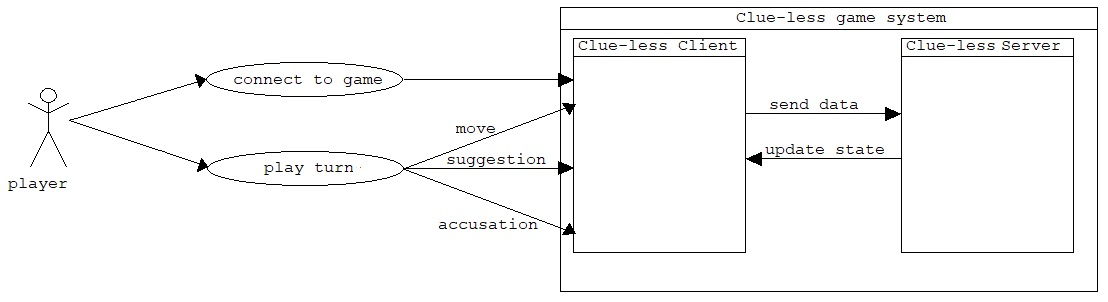
\includegraphics[width=0.9\columnwidth]{usecase1.jpg}
\caption{\label{UC1} Top level use-case diagram for the Clue-less game system}
\end{figure}

\subsection[Server Architecture]{Server Architecture}
The server requirements are detailed in Section \ref{serverReqs}.  Due to the requirements \ref{reqS.12}, \ref{reqS.2}, \ref{reqS.3}, and \ref{reqS.14} the server will need to have three modules.  The first module, the \textbf{listModule} will be responsible for listening to incoming connects, accepting the and then enqueueing the connection.  The second module, \textbf{manModule} is responsible for managing the queue and spawning a game when at least the appropriate number players are in the queue.  Finally, the \textbf{gameModule} is responsible for implementing the game logic expressed in Section \ref{gameReqs}.  The sequence of interactions in the server are shown in Figure \ref{serverSeq}.

\begin{figure}[ht]
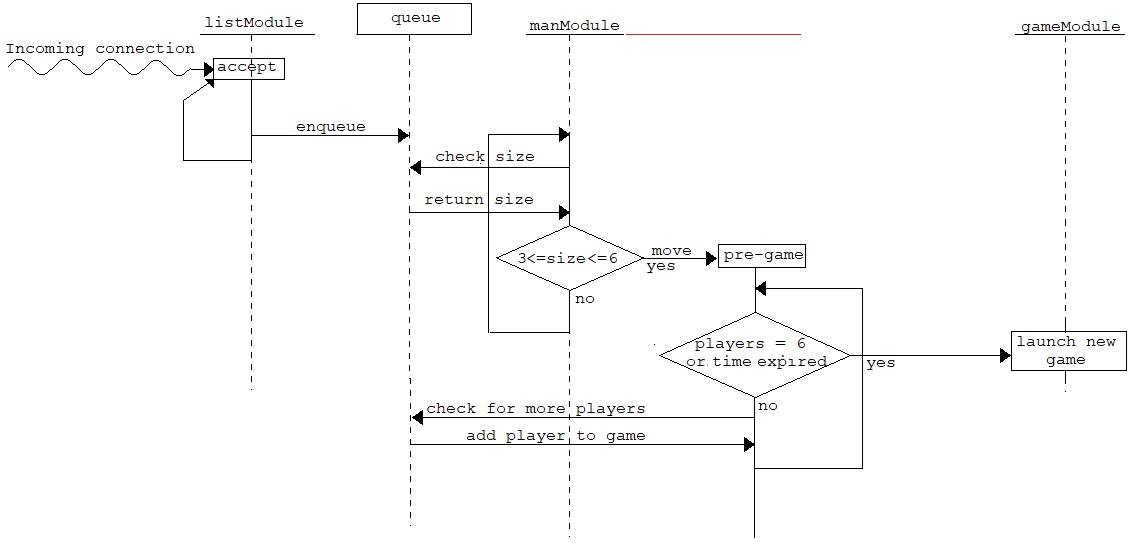
\includegraphics[width=0.9\columnwidth]{serverSequence}
\caption{\label{serverSeq} Sequence diagram for the Clue-less server}
\end{figure}

In the listening module, the main server {\em socket} is created and it is marked as passive and then \texttt{accept} is called.  This function will block till a connect attempt is made.  The server accepts the connect and enqueues it and then return back to the \texttt{accept} function.  Assuming that this module is implemented in its own thread it will be ensured that the server will remain responsive, thus meeting requirement \ref{reqS.12}.  
\par
The next module \textbf{manModule} will be responsible for managing the player queue, and will periodically check the size of the queue, and if the is at least three players in the queue, move at most six players into the pre-game holding area and start a countdown timer as described in Requirement \label{reqS.4}.  The manager module will the monitor if any new connections have been made, and add those connections to the pre-game staging area, insuring that the number of players does not exceed 6, as per Requirement \ref{reqG.2}.  Once there are the maximum number of players, or the time expires the manager will have those connects of to the game module and a new game will start.  At this time communications between the server and the clients will be managed by the game module.
\par
The final module, the \textbf{gameModule} will implement the rule of the game expressed in Section \ref{gameReqs}.  The first thing this module will do is prepare the case file as described in Requirements \ref{reqG.8} through \ref{reqG.11}.  Then the remaining cards will be distributed as described in \ref{regG.12}.  As expressed in Requirement \ref{reqG.3}, play will start with the player playing Miss Scarlet.

\subsubsection[Implementation Details]{Implementation Details}
The server will be implemented in C$^{++}$, using the standard Berkeley Socket API.  We shall provide logging capability to a default or user-configured log file.  It is expected that the server will execute without significant care and feeding.  To support testing we will provide a minimal command line interface.

\subsection[Client Architecture]{Client Architecture}

\subsubsection[Implementation Details]{Implementation Details}
The client will be implemented in C$^{++}$, using the QT library for the graphical presentation.



\pagebreak
\begin{figure}
\centering
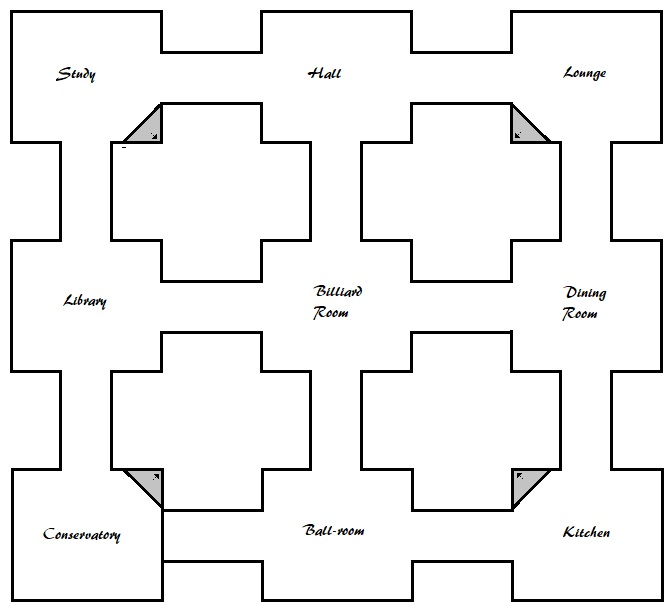
\includegraphics[width=0.9\columnwidth]{board}
\caption{\label{fig1}Clue-less board}
\end{figure}
\end{document}